%%%%%%%%%%%%%%%%%%%%%%%%%%%%%%%%%%%%%%%%%%%%%%%%%%%%%%%%%%%%%%%%%%%
%%% Documento LaTeX                                             %%%
%%%%%%%%%%%%%%%%%%%%%%%%%%%%%%%%%%%%%%%%%%%%%%%%%%%%%%%%%%%%%%%%%%%
% Título:   Apéndice A
% Autor:    Ignacio Moreno Doblas
% Fecha:    2014-02-01
% Versión:  0.5.0
%%%%%%%%%%%%%%%%%%%%%%%%%%%%%%%%%%%%%%%%%%%%%%%%%%%%%%%%%%%%%%%%%%%%

\pagestyle{fancy}
\fancyhead[LE,RO]{\thepage}
\fancyhead[RE]{Apéndice} %
\fancyhead[LO]{\nouppercase{\rightmark}}
%\fancyhead[RE]{Parte \thepart \rightmark} %

\chapterbegin{Funcionamiento de la placa auxiliar}
\label{chp:PlacaAux}
\minitoc

\section{Esquema}

\begin{figure}[h]
  \centering
    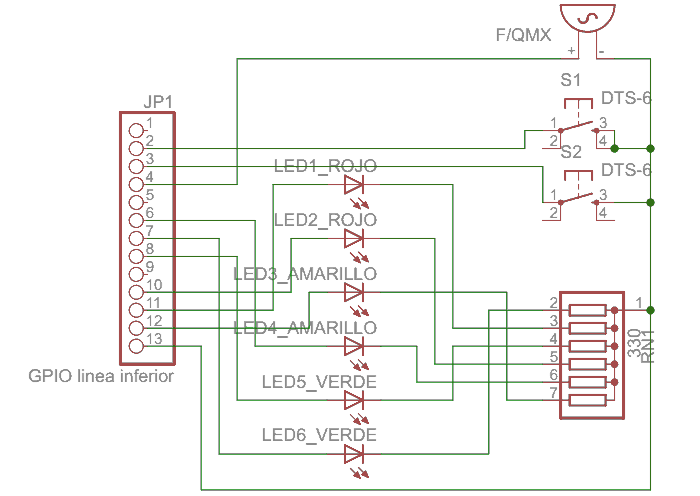
\includegraphics[width=14cm]{graphs/circuito.png}
  \caption{Esquema del circuito}
  \label{fig:circuito}
\end{figure}

Es un circuito sencillo y se puede montar en una protoboard sin
problemas, el esquema es el siguiente. Se conecta en la fila
inferior del conector GPIO, dejando libre la superior para el puerto
serie y otros propósitos.

\section{Pinout}

El puerto GPIO varía ligeramente dependiendo del modelo de Raspberry. En nuestro caso
la mayor diferencia está entre la revisión 1 y la 2, ya que el modelo B+ es compatible.
Al ser idénticos los primeros 26 pines, cualquier periférico diseñado para la revisión 2
es compatible con el modelo B+ (pero no al contrario).

La zona marcada con un recuadro verde es donde conectaremos nuestra placa auxiliar.

\begin{figure}[h]
  \centering
    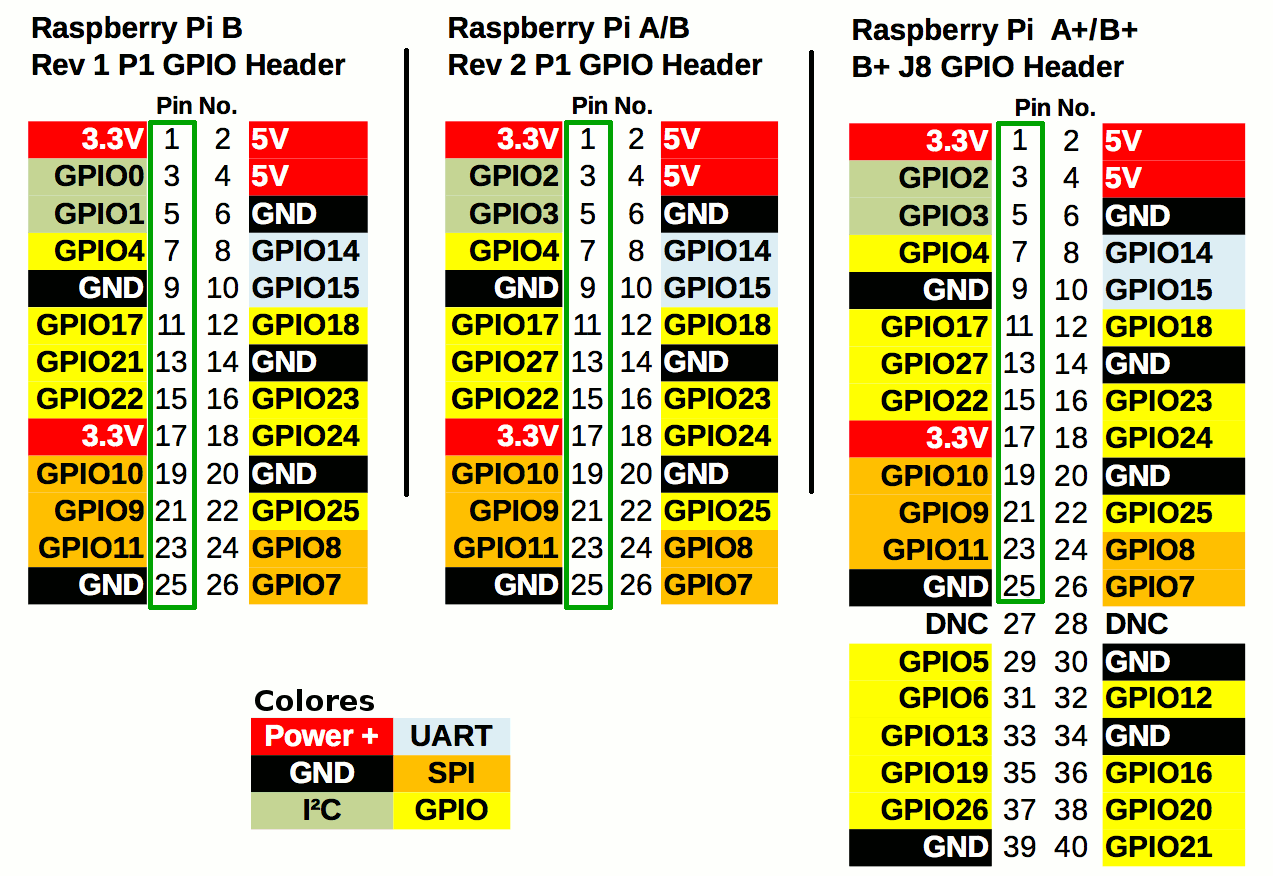
\includegraphics[width=14cm]{graphs/RaspberryGPIO.png}
  \caption{Pinout del puerto GPIO}
  \label{fig:pinout}
\end{figure}

\section{Correspondencia}

En la siguiente tabla vemos la correspondencia entre puertos del GPIO y
componentes. Los componentes son: 2 pulsadores, 6 LEDs y un altavoz
piezoeléctrico.

\begin{longtable}{ p{1.8cm} | p{1.2cm} | p{2cm} | p{5cm}}
\hline
{\bf Nombre} & {\bf GPIO} & {\bf Tipo} & {\bf Descripción} \\ \hline
LED1 & 0/2 & Salida & Diodo led color rojo \\ \hline
LED2 & 1/3 & Salida & Diodo led color rojo \\ \hline
LED3 & 17 & Salida & Diodo led color amarillo \\ \hline
LED4 & 22 & Salida & Diodo led color amarillo \\ \hline
LED5 & 10 & Salida & Diodo led color verde \\ \hline
LED6 & 11 & Salida & Diodo led color verde \\ \hline
BOT1 & 21/27 & Entrada & Pulsador izquierdo \\ \hline
BOT2 & 9 & Entrada & Pulsador derecho \\ \hline
ALT & 4 & Salida & Altavoz piezoeléctrico \\ \hline
\caption{Correspondencia entre pines y componentes}
\label{tab:berry}
\end{longtable}

\section{Funcionamiento}

Los LEDs son salidas que se activan (encienden) cuando escribimos un 1
en el puerto correspondiente. Cuando están a 0 permanecen apagados. Podemos
jugar con los tiempos de encendido/apagado para simular intensidades de luz
intermedias. Los LEDs de color rojo se corresponden con distintos puertos
según el modelo de Raspberry. Para hacer que nuestro programa funcione con
todos los modelos activaremos a la vez los distintos puertos. Por ejemplo
el LED1 se activa mediante GPIO 0 en la revisión 1.0 y con GPIO 2 en los demás
modelos. Nosotros usaremos GPIO 0 y GPIO 2 cada vez que necesitemos
encender o apagar el LED1.

El altavoz piezoeléctrico es otra salida, conectada al puerto GPIO 4. A diferencia
de los LEDs no basta un 0 ó un 1 para activarlo, necesitamos enviar una onda
cuadrada al altavoz para que éste suene. Es decir, hay que cambiar rápidamente de
0 a 1 y viceversa, además a una frecuencia que sea audible (entre 20 y 20000 Hz).

Por último tenemos los pulsadores. Al igual que con los LEDs rojos, hay que tener
en cuenta que BOT1 se corresponde con distintos puertos GPIO dependiendo del modelo
de Raspberry. Eléctricamente son interruptores que conectan el pin a masa cuando
están presionados. Cuando están en reposo los pines del GPIO correspondientes
quedan al aire, por lo que hay que activar por software las resistencias de
{\tt pull-up} si queremos niveles lógicos consistentes.

\chapterend
